\chapter{\label{chap:evaluation}Evaluation of Models Trained with Self-Supervision}

Models trained with self-supervision can be evaluated at two stages. Obviously, the accuracy of classification of given input is one way to do so. The other way is to evaluate embeddings either with loss function used for training of the encoder or visually after dimensionality reduction. All of these approaches are discussed in this chapter.

At first, the sports pose embeddings are visually analyzed in section \ref{sec:visual}. Then, section \ref{sec:evaluate-encoder} presents encoder's accuracy on validation dataset. After that, section \ref{sec:evaluate-classifier} displays accuracy of the classification itself on validation dataset and finally, this accuracy is compared to supervised model with same architecture in section \ref{sec:comparison}. Results of each evaluation are discussed in their respective sections. Experiments were done fairly and no results were cherry-picked.

\section{\label{sec:visual}Visual Analysis of Latent Space}

The latent space has well over 3 dimensions and therefore cannot be easily visualized. Typically, embeddings of more complex information such as sports pose can range from 64 to 512 dimensions. Vectors representing them usually satisfy the constraint of living on a unit hypersphere. Analysing data visually can help understand patterns in them and detect emerging problems. When the dimensionality is decreased to only 2 dimensions, a lot of information can be lost. Therefore, the challenging task for the projecting algorithm is to drop the non-necessary information and preserve the patterns in data.

The elemental method for dimension reduction is Principal Component Analysis (PCA). It computes a new basis of the vector space to maximize the data variance. After projecting the data into the new basis, only 2 or 3 dimensions with the highest variance can be taken into account and the rest is ignored. Finally, such data can be plotted and reviewed. Other possible projection is Linear Discriminant Analysis (LDA) that also takes into account the label of each data point and is trying to find basis that allows for the best linear separation of classes.

Whereas the previously mentioned algorithms allowed for computing the precise results, more complex methods for dimension reduction are based on iterative approaches to find the best approximation of the ideal state since it cannot be computed directly. Widely used algorithm for this task is t-distributed Stochastic Neighbor Embedding (t-SNE). It puts data points into pairs and tries to attract those that are similar and repel the dissimilar ones. Other iterative method is Uniform Manifold Approximation and Projection (UMAP) which also non-linearly projects data into 2D or 3D. I chose to use t-SNE as the dimensionality reduction algorithm because it was able to find patterns in the data embeddings better than the other algorithms.

\subsection{Dimensionality Reduction with t-distributed Stochastic Neighbor Embedding}

t-distributed Stochastic Neighbor Embedding (t-SNE) is a non-linear dimensionality reduction method suited for displaying embedding vectors in two or three-dimensional space \cite{tsne-vandermaaten08a}. It is based on Stochastic Neighbor Embedding (SNE) but it uses also t-distribution instead of only Gaussian distribution \cite{sne-NIPS2002_6150ccc6}. t-distribution has heavier tails in comparison to Gaussian distribution and therefore, it solves one of the problems of SNE, which was centering the data points into one place in the low dimensions and not preserving the gaps between them.

t-SNE algorithm starts with a random initialization of projected data points in the targeted 2 or 3-dimensional space. It places them fairly close to each other to allow for patterns emerging in higher scale. Then two similarity distributions are constructed -- one from points in the source high-dimensional space, the other from points in the destination low-dimensional space. Both distributions are constructed from distances between all pairs of data points in their respective spaces. Then, Kullback-Leibler divergence of joint distribution P in the high-dimensional space and Q in the low-dimensional space is minimized:

\begin{equation}
    \label{eq:tsne-kl}
    C = KL(P||Q) = \sum \limits_{i} \sum \limits_{j} p_{i j} \log \frac{p_{i j}}{q_{i j}}.
\end{equation}

Distances of data points from themselves $p_{i i}$ and $q_{i i}$ are set to zero. $p_{i j}$ and $p_{j i}$ are averaged in order to preserve symmetry $p_{i j} = p_{j i}$. Each data point pair is assigned a probability from Gaussian distribution with mean set to coordinates of point $i$ and variance computed from the density of other points around it. The distance of point $j$ from $i$ is projected to the Gaussian distribution and $p_{i j}$ equals the given probability, calculated as:

\begin{equation}
    \label{eq:tsne-p}
    p_{i j} = \frac{e^{-|| {y}_{i} - {y}_{j} ||^2}}{\sum \limits_{k \neq l} e^{-|| {y}_{k} - {y}_{l} ||^2}}.
\end{equation}

\noindent Probabilities $q_{i j}$ are obtained from Student's t-distribution with one degree of freedom with a similar approach to the $p_{i j}$. The formula is as follows:

\begin{equation}
    \label{eq:tsne-q}
    q_{i j} = \frac{(1 + || {y}_{i} - {y}_{j} ||^2)^{-1}}{\sum \limits_{k \neq l} (1 + || {y}_{i} - {y}_{j} ||^2)^{-1}}.
\end{equation}

\noindent Finally, gradient of the Kullback-Leibler divergence between P and Q is computed with:

\begin{equation}
    \label{eq:tsne-gradient}
    \frac{\partial C}{\partial y_{i}} = 4 \sum \limits_{j} (p_{i j} - q_{i j}) (y_{i} - y_{j}) (1 + || {y}_{i} - {y}_{j} ||^2)^{-1}.
\end{equation}

\subsection{Analysis of embeddings with t-distributed Stochastic Neighbor Embedding}

The encoder presented in section \todo{number} transforms image of sports pose into 256-dimensional vector embedding. The goal is to have this embedding describe only the sports pose and ignore background of the scene and look of the person doing the pose. Sports poses similar to each other should be closer to each other in the embedding space than poses that are completely different. If only one arm moved from one image frame to another, their embeddings should be very similar. The same pose performed by other person in a different place and even photographed from a different angle should have the same or at least very similar embedding.

The whole \todo{name} dataset introduced in section \todo{number} includes 3804 divided into 4 classes according to arm positions of the person -- each arm is either pointing down or up and therefore, the corresponding classes are named \texttt{down-down}, \texttt{down-up}, \texttt{up-down} or \texttt{up-up}. Positions where both arms are in a downward direction should be relatively far from each other while the other 2 classes can be placed somewhere in between the edge cases. The dataset consists of 10 scenes, each filmed from 3 angles. Projected embedding are displayed in the figure \ref{fig:t-sne}.

\begin{figure}[!ht]
    \centering
    \begin{tikzpicture}
        \pgfplotsset{scale=1.5}
        \begin{axis}[
            title={Embeddings of sports poses after t-SNE projection},
            xlabel={x},
            ylabel={y},
            legend pos=outer north east,
            xmajorgrids=true,
            ymajorgrids=true,
            grid style=dashed,
        ]
            \addplot[
                only marks,
                color=yellow,
                mark=+,
                mark options={scale=0.7}
            ]
                table[col sep=comma, header=true] {figures/t-sne/down-down.csv};
            \addplot[
                only marks,
                color=orange,
                mark=+,
                mark options={scale=0.7}
            ]
                table[col sep=comma, header=true] {figures/t-sne/down-up.csv};
            \addplot[
                only marks,
                color=red,
                mark=+,
                mark options={scale=0.7}
            ]
                table[col sep=comma, header=true] {figures/t-sne/up-down.csv};
            \addplot[
                only marks,
                color=purple,
                mark=+,
                mark options={scale=0.7}
            ]
                table[col sep=comma, header=true] {figures/t-sne/up-up.csv};
            \legend{down-down, down-up, up-down, up-up}
        \end{axis}
    \end{tikzpicture}
    \caption{Embeddings of all 3804 samples from the \todo{name} dataset projected from 256 dimensions to 2D with the t-SNE algorithm. Data points are colored according to their class. Parameters of the t-SNE were 600 iterations, perplexity 16, learning rate 10 and the algorithm ran without any supervision based on sample labels.}
    \label{fig:t-sne}
\end{figure}

The projection clearly shows a number of clusters of different sizes, each consisting of data points from all 4 classes. Each cluster is probably a representative of single viewpoint of a scene with some of them being closer to each other or even almost merged together. This shows that the encoder model is not capable of generalizing over different scenes nor viewpoints. One possible explanation of such behaviour is not using diverse enough dataset.

When focusing on each cluster individually, the data point distribution holds relations for similar sports poses. Classes \texttt{down-down} and \texttt{up-up} are usually far apart from each other within the cluster and while the \texttt{down-up} and \texttt{up-down} are between them. Some images of poses contain arms pointing almost perfectly horizontally and their classification cannot be precise. These cases have to be taken into account.

\section{\label{sec:evaluate-encoder}Evaluation of Encoder on Validation Dataset}

\section{\label{sec:evaluate-classifier}Evaluation of Classifier on Validation Dataset}

\section{\label{sec:comparison}Comparison of Self-Supervised and Supervised-Trained Models}

The main advantage of models trained in a self-supervised manner is their ability to perform well with dataset containing smaller number of labeled data than what would supervised training needed. This advantage is shown in evaluation done on different-sized datasets in the following experiment.

The model described in the previous chapter (\todo{chapter link}) is used as the self-supervised learning benchmark. For supervised learning representative the ResNet50 model is chosen and it is not alternated in any way \cite{he2015deep}. The architectures of both networks are very similar as can be seen in the table \ref{tab:self-supervised-vs-supervised}, their backbones are the same, only their last few layers are different, and therefore, the evaluations should not be distorted because of the models.

\begin{table}[!ht]
    \begin{center}
        \begin{tabular}{ |c|c||c|c| }
            \hline
                \multicolumn{2}{|c||}{Self-Supervised Model} & \multicolumn{2}{c|}{Supervised Model} \\
            \hline
            \hline
            Description & Layer -- Shape & Layer -- Shape & Description \\
            \hline
            \hline
                Image & Input -- (224, 224, 3) & Input -- (224, 224, 3) & Image \\
            \hline
                \makecell{Backbone \\ ResNet50} & \makecell{Padding -- (230, 230, 3) \\ \vdots \\ Pooling -- (2048)} & \makecell{Padding -- (230, 230, 3) \\ \vdots \\ Pooling -- (2048)} & \makecell{Backbone \\ ResNet50} \\
            \hline
                & Dense -- (256) & \multirow{4}{*}{Dense -- (4)} & \multirow{4}{*}{Label} \\
            \cline{1-2}
                Embedding & L2 Normalize -- (256) & & \\
            \cline{1-2}
                & Dense -- (64) & & \\
            \cline{1-2}
                Label & Dense -- (4) & & \\
            \hline
        \end{tabular}
    \end{center}
    \caption{Comparison of architectures of self-supervised and supervised models. Their input, backbone and output are identical, only the top of self-supervised model is adjusted for the self-supervised training.}
    \label{tab:self-supervised-vs-supervised}
\end{table}

Since each model is trained in a different way, it is not trivial to set the borderline for number of epochs used for training. For that reason, each model was trained for sufficient number of epochs after which it no longer improved on validation data. The self-supervised model consists of two parts -- the encoder which creates the embedding from an image and the recognizer which classifies the pose from the embedding. The encoder was trained for 30 epochs and the recognizer for 20 epochs. The encoder was trained once and stayed the same for the whole experiment while the recognizer was fitted for every dataset sample. The supervised model was trained for 50 epochs on each dataset sample.

Dataset used for this experiment is thoroughly described in section \ref{sec:basic-dataset}. It contains 3804 images of 1268 poses, each captured from 3 different angles. The poses are not necessarily unique but the images differ in background and clothes of the person. Overall, there are 10 different scenes with 2 possible backgrounds and different clothing of the person in each of the scenes. The poses represent possible movements of person's arms in all directions and joints' bendings, other parts of the body such as torso, head or legs are not moving. Each image belongs to one of 4 classes that differ in position of arms -- left or right arm is pointing either down or up. Since some positions may be questionable, the rule of thumb during labeling of data was whether the wrist is above or below the corresponding shoulder.

Both of tested models were fitted on datasets of different sizes and then their accuracy on never-seen validation data was evaluated. Before each training the whole dataset was shuffled and then divided into training and validation subsets. The portion of data used for training was the changing variable and it ranged from $0.9$ to $0.025$. The rest of the data where always used for validation. This approach decreases variance in the training dataset and concurrently increases it in the validation dataset. Because of this, model's ability to generalize well is displayed.

To keep the experiment fair, dataset for each experiment was shuffled with the same seed for both models and, therefore, they had the same data for training and evaluating. For each dataset split portion, 10 runs of fitting and evaluating were done, each one with different seed. Seeds were chosen deterministically as integers from $0$ to $9$. Accuracy on validation data was then averaged over all 10 runs to get the final accuracy of the model for a given fraction of training data.

The results of the evaluation are shown in the figure \ref{fig:self-supervised-vs-supervised}. For training dataset portions down to $15 \%$ (which equals $570$ of the $3804$ images used for training), the performances of self-supervised and supervised models are on a par. When the training dataset portion decreases to $12.5 \%$ ($475$ of $3804$ images) the supervised model starts to degrade and with just $2.5 \%$ images it approaches accuracy $25 \%$ which is for 4 classes basically a random guess. While the self-supervised model keeps its accuracy above $60 \%$ even when trained on $2.5 \%$ data which equals to $95$ images for training and $3709$ for validation.

\begin{figure}[!ht]
    \centering
    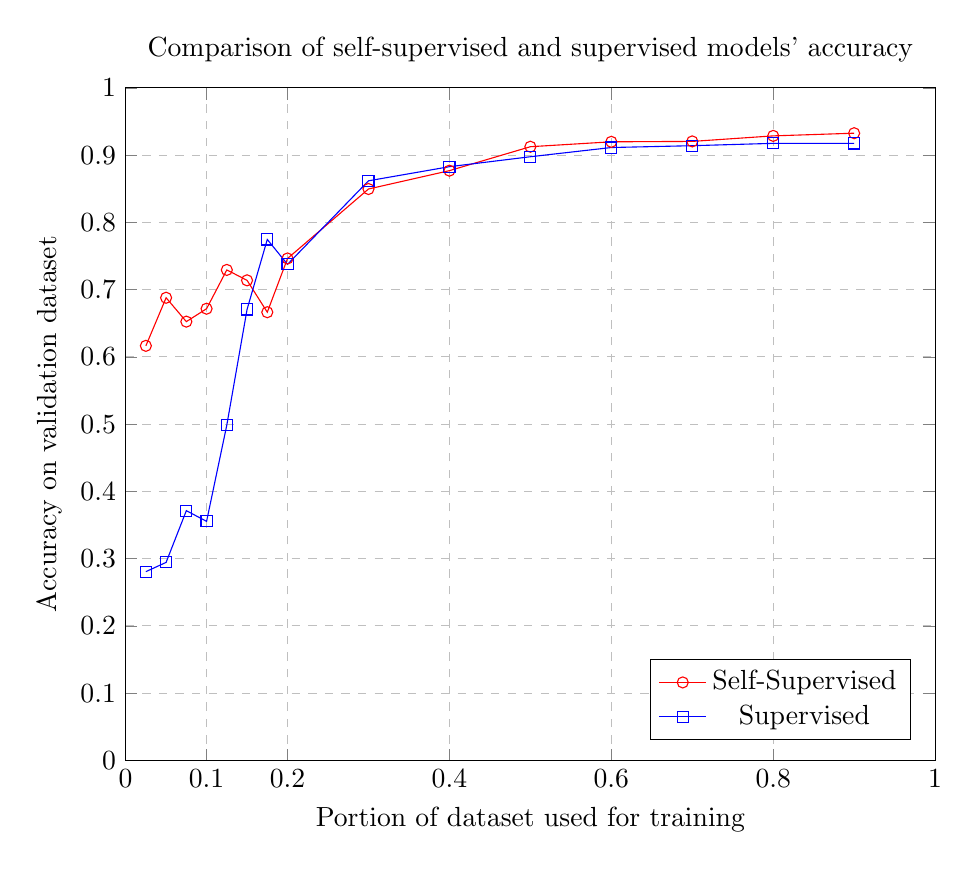
\begin{tikzpicture}
        \begin{axis}[
            title={Comparison of self-supervised and supervised models' accuracy},
            xlabel={Portion of dataset used for training},
            ylabel={Accuracy on validation dataset},
            xmin=0, xmax=1,
            ymin=0, ymax=1,
            xtick={0,0.1,0.2,0.4,0.6,0.8,1},
            ytick={0,0.1,0.2,0.3,0.4,0.5,0.6,0.7,0.8,0.9,1},
            legend pos=south east,
            xmajorgrids=true,
            ymajorgrids=true,
            grid style=dashed,
        ]
            \addplot[color=red,mark=o]
                coordinates {(0.025,0.6164)(0.050,0.6879)(0.075,0.6524)(0.100,0.6716)(0.125,0.7293)(0.150,0.7138)(0.175,0.6664)(0.200,0.7463)(0.300,0.8496)(0.400,0.8769)(0.500,0.9125)(0.600,0.9198)(0.700,0.9204)(0.800,0.9286)(0.900,0.9326)};
            \addplot[color=blue,mark=square]
                coordinates {(0.025,0.2806)(0.050,0.2944)(0.075,0.3713)(0.100,0.3554)(0.125,0.4986)(0.150,0.6705)(0.175,0.7746)(0.200,0.7376)(0.300,0.8618)(0.400,0.8828)(0.500,0.8976)(0.600,0.9113)(0.700,0.9140)(0.800,0.9175)(0.900,0.9174)};
            \legend{Self-Supervised, Supervised}
        \end{axis}
    \end{tikzpicture}
    \caption{Performance of self-supervised and supervised models on validation dataset based on what fraction of the whole dataset was used for training. The rest of the dataset was used for validation. Each datapoint is an average of 10 runs. Self-supervised model displays better accuracy for small training datasets. With the dataset size getting larger, both models perform similarly.}
    \label{fig:self-supervised-vs-supervised}
\end{figure}
